\chapter{Background}
\label{chap:background}
This chapter provides context to the underlying research. Section \ref{sec:msa_intro} presents MSA. Key concepts about Deep Learning (\acrshort{dl}) models utilized in this study are described in Section \ref{sec:dl_models}. COGMEN, which is the state-of-the-art MSA model and widely used in this Master's thesis research, is presented in Section \ref{sec:COGMEN}. Section \ref{sec:emotions} entails basic abstractions of emotion theory. Lastly, Section \ref{sec:big-five_model} presents the Big Five personality model. 

\section{Multimodal sentiment analysis}
\label{sec:msa_intro}
In traditional sentiment analysis, emotions are retrieved from textual information. MSA aims to generalize the standard text based sentiment analysis to videos where three communicative modalities are present: text, video, and acoustics. This focus on MSA is essential to understand human behavior, because human communication occur through both verbal and nonverbal cues. Therefore, when someone utters a sentence, the meaning of the utterance can drastically shift depending on the nonverbal behaviours. For example, the sentence \say{The movie is sick.} is ambiguous when perceived from a textual perspective because it can be considered both positive and negative. When the utterance is combined with a smile, the sentence will automatically become positive. When the speaker says the same sentence with a frown expression, it will be negatively loaded. A person speaking \say{The movie is sick.} in a loudly voice will also be ambiguous. This means that visual features are powerful in describing something more effectively than words and can in particular be used to predict a sentiment with textual data. MSA systems may consist of a combination of two modalities such as text+video, text+speech, speech+video, or all three. A system including two modalities is called a bimodal system whereas a system with all three modalities present is called a trimodal system. \\

Modalities come in different forms including audio i.e. vocal words (e.g. utterances, tones, laughs), visual features (e.g. gestures, eye contact), and text (e.g. transcripts produced from audio data), or in the form of electroencephalography (\acrshort{eeg}) signals \cite{MSA-review-3-9686504}. The text comprises of polar words where only a subset of the words contribute to the sentiment. It is also divided into word group or phrases, character N-Grams, and phoneme N-Grams in order to understand the context of the given text. Audio features are for example pitch, pauses, intonation, energy distribution over a sentence, and speed of an utterance. The visual indicators include smiles, frowns, gestures, posture, gazes, and eye contact. \\

Figure \ref{fig:msa_process} illustrates the general process of MSA by fusing several modalities. First, the unstructured data such as a video is taken as input and then pre-processed. In the pre-processing phase, data is cleaned and filtered into audio, video, and textual data using various dimensionality reduction techniques. Then, features from audio, visual, and textual data is extracted using different feature methods.  
%
\begin{figure}[h]
  \centering
  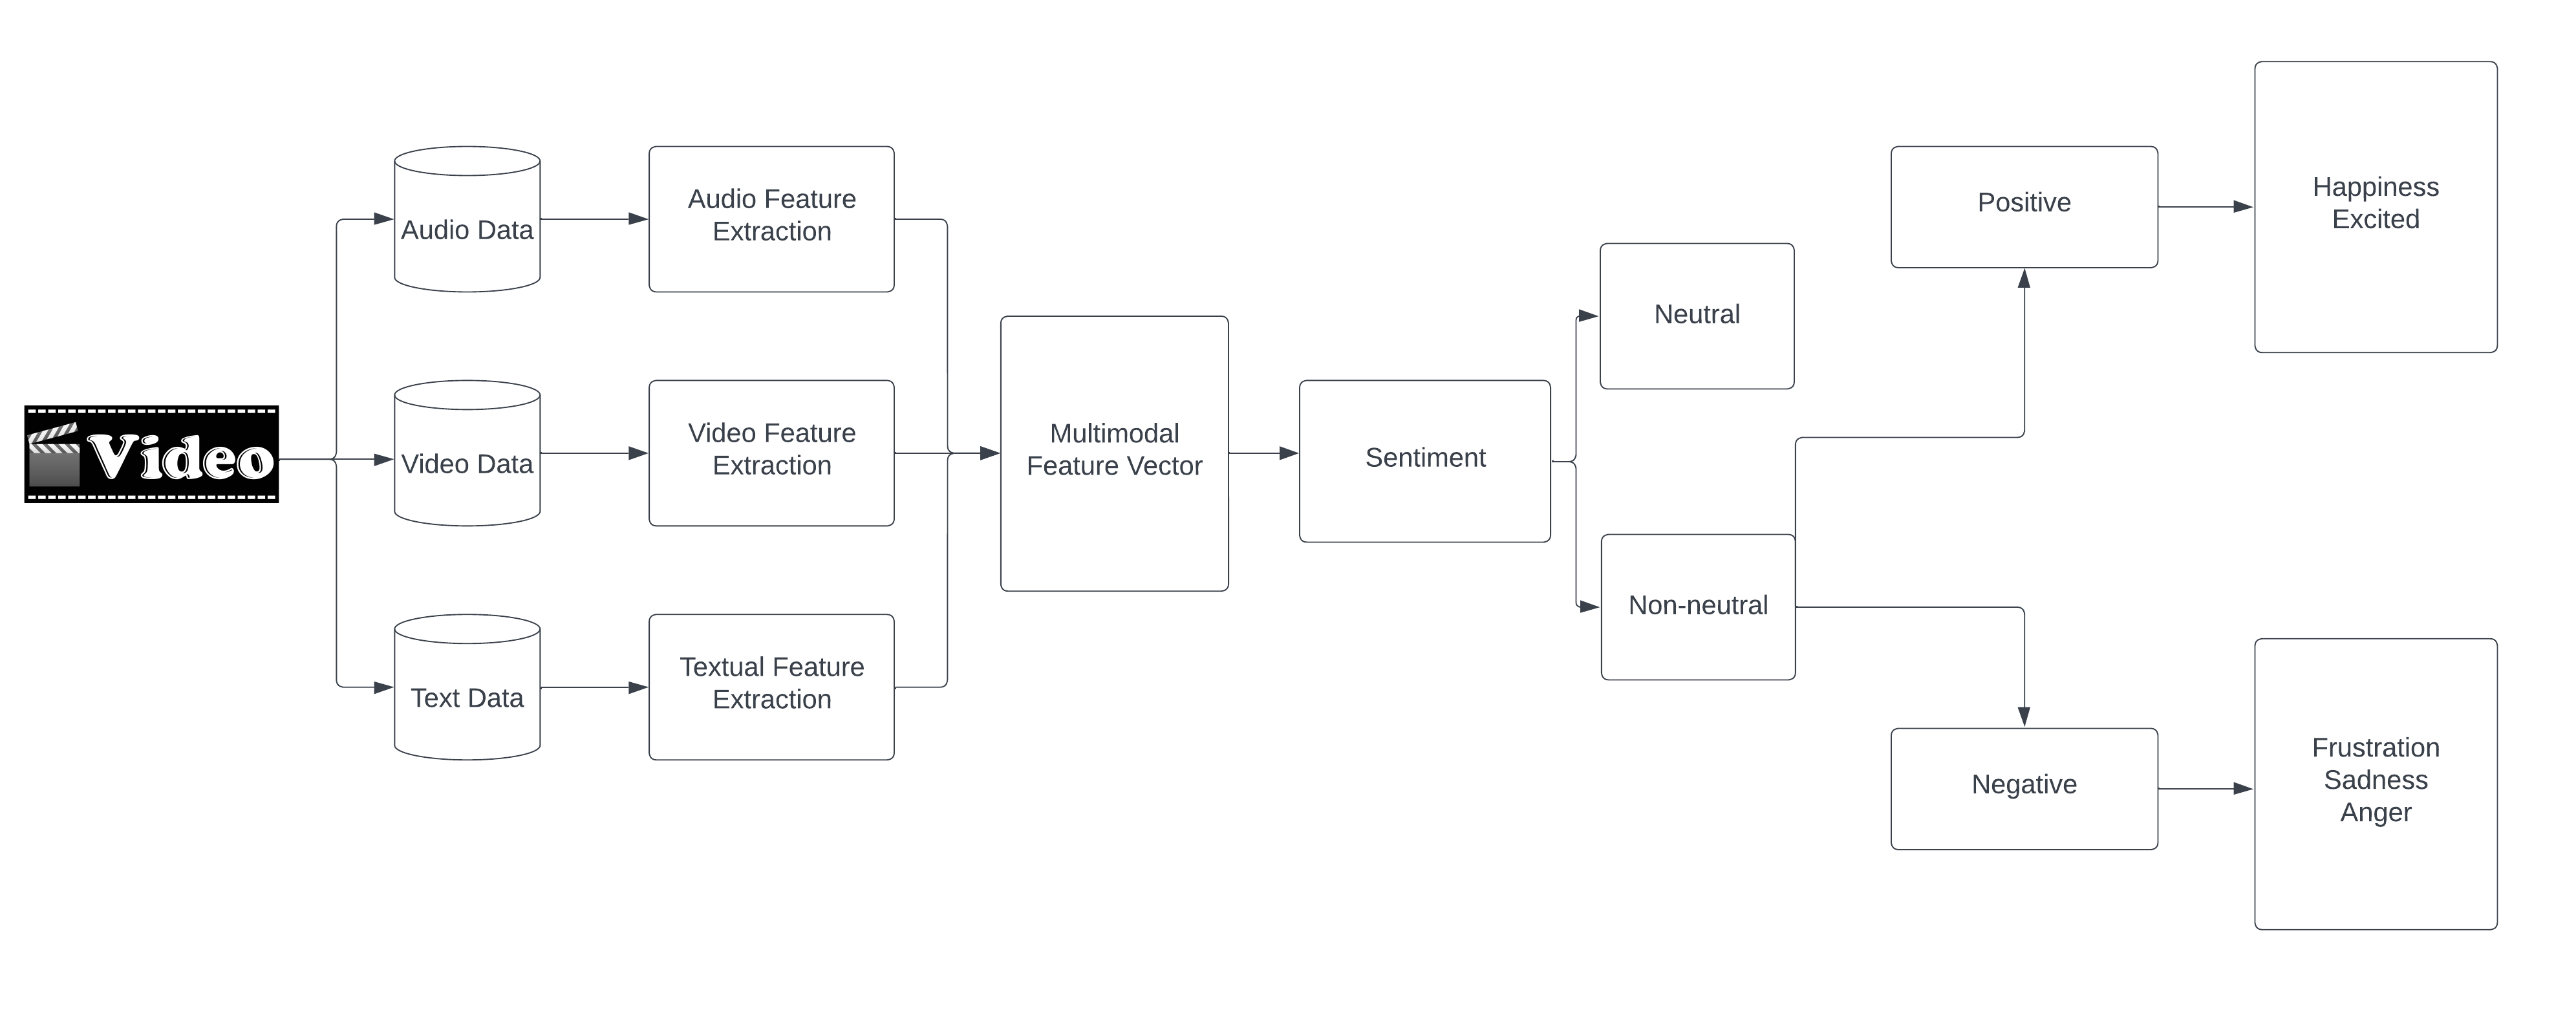
\includegraphics[width=\textwidth]{figures/msa_process_dpi.png}
  \caption{MSA process.}
  \label{fig:msa_process}
\end{figure}
%
From the feature extraction phase, feature vectors are converted into a decision feature vector for multiple modalities. Lastly, a classification algorithm categorizes the corresponding sentiment/emotion based on the multimodal feature vector. Sentiments can be classified as neutral and non-neutral. A neutral emotion denotes that no feelings are expressed to any circumstances. The non-neutral category consists of positive and negative emotions. Emotion classification can also be more fine-grained, where positive and negative emotions are divided into emotion classes (i.e. happy and excited for positive emotions and frustration, sadness, and anger for negative emotions). This thesis is limited to five primary emotions - happy, excited, frustration, sadness, and anger. Additionally, the neutral emotion is important. \\

The most critical activity of MSA is fusion of multiple modalities. Fusion is the process of combining, filtering and extracting required features from the data accumulated from different modalities \cite{MSA-review-3-9686504}. Multimodal fusion is important because this data is used to classify the emotions. Currently, there are ten different multimodal fusion architectures:
%
\begin{itemize}
    \item \textbf{Early fusion-feature level fusion}: Feature level fusion, also called early fusion, merges the extracted features from visual, audio, and textual data into a high dimensional feature vector \cite{MSA_review2_GANDHI2023424}. Then, it is processed in the desired classification algorithm. \\
    \item \textbf{Late fusion-decision level fusion}: In late fusion, the features of each modality is examined and classified independently before the results are fused together to form a final decision vector that predicts the emotion \cite{MSA-review-3-9686504}. \\
    \item \textbf{Hybrid fusion}: Hybrid fusion utilizes both early and late fusion for emotion classification. When using hybrid fusion, the benefits of early and late fusion is exploited while their drawbacks are excluded at the same time \cite{MSA-review-3-9686504}.\\
    \item \textbf{Model-level fusion}: The characteristics of each modality is examined to find the correlation between them. The model is then developed in accordance with the research domain and given problem requirements \cite{MSA-review-3-9686504}. \\
    \item \textbf{Tensor fusion}: With the use of a tensor fusion layer that explicitly imitates unimodal, bimodal, and trimodal interactions, this method creates a 3-fold Cartesian product. It reduces the quantity of training samples needed \cite{MSA_review2_GANDHI2023424}. \\
    \item \textbf{Hierarchical fusion}: As the name indicates, this fusion process fuses the features in an hierarchical order. Here, the model starts to merge the modalities two in two first, and then all three modalities \cite{MSA_review2_GANDHI2023424}. \\
    \item \textbf{Bimodal fusion}: In bimodal fusion, two different modality pairs are used as input to deal with the information imbalance between modalities. The two components are trained concurrently so they can duel in a simulated combat \cite{MSA_review2_GANDHI2023424}. \\
    \item \textbf{Attention mechanism-based fusion}: Attention mechanism-based fusion aims to incorporate multi-level contextual feature extraction. To do this, the model uses attention-based inter-modality fusion at utterance level since each modality contributes differently to sentiment and emotion classification. Contextual attentive unimodal features are joined two by two to create bimodal features. These two sets of features are then combined to form trimodal feature vectors \cite{MSA_review2_GANDHI2023424}. \\
    \item \textbf{Quantum based fusion}: In this method, quantum inference is used to capture the interactions within each utterance (i.e. correlations between different modalities). Additionally, quantum measurement is used to build a strong-weak influence model to find the interactions between consecutive utterances (i.e. how one speaker is influenced by another). Quantum based fusion also utilizes decision-level or early fusion techniques \cite{MSA-review-3-9686504}. \\
    \item \textbf{Word level fusion}: This method investigates the interplay between different modalities in order to establish a superior sentiment tendency. Transformers are used to learn joint representations for utterances and to translate across different modalities \cite{MSA_review2_GANDHI2023424}. 
\end{itemize}

\section{Deep learning models}
\label{sec:dl_models}
Deep Learning models for emotion recognition are utilized in this research. A deep neural network (DNN) comprises an input, output, and a set of hidden layers with multiple nodes or neurons. For each layer $l$ in the network, the output layer is computed as follows:
%
\begin{equation*}
    h^{l} = f(W^{l} \cdot h^{l-1} + b^{l}),\tag{1}
\end{equation*}
%
where $W^{l}$ is the weight matrix connecting the $l-1^{th}$ to the $l^{th}$ layer. $b^{l}$ is the bias for the $l^{th}$ layer, and $f$ is the non-linear activation function (e.g. sigmoid, hyperbolic tangent, rectified linear unit (ReLU), etc.). The output of the last layer $y^{L}$ is the output of the last activation function:
%
\begin{equation*}
    y^{L} = f(W^{L} \cdot h^{L-1} + b^{L}). \tag{2}
\end{equation*}
%
The linear transformation in each layer can be expressed as a matrix multiplication:
%
\begin{equation*}
    W^lh^{l-1} = W^l {*} h^{l-1},\tag{3}
\end{equation*}
%
where $*$ denotes matrix multiplication and $h^{l-1}$ is the output of the previous layer. Weights and biases are adjusted usually using backpropagation during training. The backpropagation is an expression for the partial derivative $\frac{\partial C}{\partial w}$ of the cost function \textit{C} with respect to any weight \textit{w} (or bias \textit{b} ) in the network \cite{cross_cultural}. The quadratic cost function can be defined as:
%
    \begin{equation*} C = \frac {1}{2n}\sum _{x}^{} \left \|{ y(x) - \alpha ^{L}(x) }\right \|^{2},\tag{4}\end{equation*}
%
where $n$ is the total number of training examples, $x$ is the training samples, $y=y(x)$ is the corresponding desired output, $L$ denotes the number of layers in the network, and $\alpha ^{L} = \alpha ^{L}(x)$ is the vector of activations output from the network when $x$ is input.

\subsection{Convolution Neural Networks}
Convolutional Neural Networks (\acrshort{cnn}s) consist of multilayers of fully connected layers. That means, each neuron in the network is connect to all neurons in the next layer. The first layer of the network is called the convolutional layer. It applies a set of filters to the input data. Each filter is a small window of weights that is convolved with the input data to produce a feature map. The operation of 2-dimensional convolution can be represented as:
%
\begin{equation*}s(i,j)=(I*K)(i,j)=\sum \limits _{l}{\sum \limits _{m}{I(l,m)K(i+l,j+m)}},\tag{5}\end{equation*}
%
where \textit{I} is a two-dimensional input matrix, and \textit{K} is a two-dimensional kernel matrix. \textit{s} denotes the resulting feature map after the convolution.

\subsection{Graph Neural Networks}
A Graph Neural Network (\acrshort{gnn}) is used to operate graph-structured data. A GNN model consists of a graph $G$ with $N$ nodes and an adjacency matrix $A$ that represents the edges between nodes. Each node $i$ has an associated feature vector $x_{i}$ with dimension $D$, and the output of the GNN for node $i$ is denoted as $y_{i}$. A linear transformation is applied to each node's feature vector to produce a hidden state vector $h_{i}$:
%
\begin{equation*}
    h_{i} = Wx_{i}x_{i},\tag{6}
\end{equation*}
%
where $W$ is the weight matrix for the linear transformation. The hidden state vectors of the neighbouring nodes are aggregated using the following message passing function:
%
\begin{equation*}
    m_{i} = {\sum \limits _{j}} A_{ji}h_{j},\tag{7}
\end{equation*}
%
where $m_{i}$ is the message node \textit{j} to node \textit{i}, and $A_{j}$ is the element of the adjacency matrix representing the edge between node $j$ and $i$. Next, the message is passed through a non-linear activation function $f$:
%
\begin{equation*}
    m_{i} = f(m_{i}).\tag{8}
\end{equation*}
%
The aggregated message for node $i$ is then combined with the hidden state of the node to produce a new hidden state as shown in Equation \ref{eq:new_hidden}.
%
\begin{equation*}
    \label{eq:new_hidden}
    h_{i'} = f(Wx_{i}h_{i} + m_{i}) \tag{9}
\end{equation*}
%
To allow for information propagation between nodes in the graph, this process can be repeated multiple times. Final output of the GNN for each node can be computed by applying another linear transformation to the final hidden state as follows:
%
\begin{equation*}
    y_{i} = W'h_{i},\tag{10}
\end{equation*}
%
where $W'$ is the weight matrix for the output transformation. Similar to a DNN, the parameters of the GNN are altered using backpropagation to minimize the loss function.

\subsection{LSTM}
This thesis also employs Long Short-Term Memory (\acrshort{lstm}). LSTM is a type of RNN that addresses the vanishing gradient problem by introducing memory cells and gates \cite{_LSTM_10.1162/neco.1997.9.8.1735}. LSTMs are designed to capture long-term dependencies in sequential data, making them effective for tasks such as speech recognition and language translation. Unlike traditional RNNs, LSTMs have a more complex architecture with memory cells and gates that control the flow of information. These gates, including the input gate, forget gate, and output gate, regulate the information flow into and out of the memory cell. This allows LSTMs to selectively remember or forget information over long sequences, enabling the network to carry relevant information forward in time. Mathematically, the process of carrying memory forward in an LSTM can be expressed as follows:
\begin{equation*}
    C_{t} = f_{t} \odot C_{t-1} + i_{t} \odot \Tilde{C}_{t},\tag{11}
\end{equation*}
%
where $C_{t}$ represents the cell state at time step \textit{t}, $f_{t}$ is the forget gate, $C_{t-1}$ is the previous cell state, $i_{t}$ is the input gate, and $\Tilde{C}_{t}$ is the candidate cell state. The $\odot$ denotes element-wise multiplication.

\subsection{Transformers}
The use of transformers have improved the performance of natural language processing tasks. In contrast to recurrent neural networks (RNN) and CNNs which operate on sequences of input data, transformers can process sequences of various length. There are two main components which constitutes the transformer architecture: the encoder and the decoder. Both components are composed of multiple layers of self-attention and feed-forward neural networks \cite{transformers1-vaswani2017attention}. Self-attention is a mechanism that allows the model to weigh the importance of different elements in the input sequence. It computes a weighted sum of the input sequence elements, where the weights are determined by the similarity between query, key, and value vectors.  The self-attention mechanism can be expressed as shown in Equation \ref{eq:transformers}.
%
\begin{equation*}
    \label{eq:transformers}
    \text{Attention}(Q,K,V) = \text{softmax}(\frac{QK^{T}}{\sqrt{d_{k}}})V,\tag{12}
\end{equation*}
%
where \textit{Q}, \textit{K}, and \textit{V} are the query, key, and value matrices, respectively. $d_{k}$ denotes the dimensionality of the key vectors. The \textit{softmax} function is utilized to ensure attention weights sum to one. In the encoder, the input sequence is fed through the self-attention layer and the feed-forward layer. The output of each layer is then passed to the next. Output of the encoder can be represented as follows:
%
\begin{equation*}
    \text{Encoder}(x)=\text{LayerNorm}(x + \text{SelfAttention}(x) +\text{FeedForward}(x)),\tag{13}
\end{equation*}
%
where $x$ is the input sequence and the \textit{LayerNorm} function is used to normalize the output of each layer. For the decoder, the self-attention layer is modified to include an additional attention mechanism that allows the decoder to attend the encoder's output. This method is referred to as encoder-decoder attention. The decoder output can be expressed mathematically as:
%
\begin{equation*}
    \resizebox{0.9\hsize}{!}{$%
    \text{Decoder}(y, \text{Encoder}(x)) = \text{LayerNorm}(y + \text{SelfAttention}(y) + \text{EncoderDecoderAttention}(y, \text{Encoder}) + \text{FeedForward}(y)),\tag{14}
    $}%
\end{equation*}
%
where $y$ is the input sequence in the decoder and the \textit{EncoderDecoderAttention} function calculates the attention weights between the decoder input sequence and the encoder output sequence. 

\section{COGMEN}
\label{sec:COGMEN}
The Contextualized Graph neural network based Multimodal Emotion recognition (\acrshort{cogmen}) model is the main MSA utilized in the thesis. It focuses on exploiting contextual information, inter-speaker and intra-speaker relations in one-sided as well as multiparty conversation settings \cite{COGMEN_joshi-etal-2022-cogmen} \cite{HP_Advanced}. This means that the framework addresses key concepts to capture emotions in a conversation: It leverages the overall context in the dialogue referred to as the global information. Also, it utilizes the local information stored in the conversations to monitor the emotion expressed by each speaker and create relations between the syllables. In essence, COGMEN is made up of four different modules that are responsible of predicting the emotion of an input utterance. The first module is called Context Extractor. Each input utterance consist of concatenated features from visual, acoustic, and textual modalities. The Context Extractor utilizes a transformer encoder in capturing the global information from each input utterance. With newly established context features, these attributes are fed into the second module, Graph Formation. This unit forms the features to a graph where each statement act as a node of the graph and they are connected using directed relations. Here, there exist two type of relations: relation between utterances by the same speaker (intra-relations) and relations between utterances from different speakers (inter-relations). Next, the third model is Relational GCN (RGCN) and GraphTransformer. The RGCN uses the graph as input to capture intra-speaker and inter-speaker dependencies. Then, the GraphTransformer supplements the RGCN by extracting rich representations from the node features by considering nodes that are connected via edges. Lastly, the fourth module is the Emotion Classifier. Based on features extracted in the previous step, a linear classifier is utilized to predict the emotion for each utterance.

\section{The use of AVIs in e-recruitment}
As young people are staying in education longer than ever, they become very attractive in the labour market. Everyone desires to get their dream job, and selecting the best candidates that fit well with the job description is essential to meet the employer's expectations. Like every other aspect with business today, the hiring process depends on speed and accuracy \cite{hiring-process-Sołek-BorowskaWilczewska+2018+25+33}. The job market has become more competitive due to an increasing number of highly relevant candidates competes against a decreasing pool of jobs. Additionally, the selection process is relatively short meaning that the hiring managers have to precisely choose the most suited candidates. The integration of both software and hardware in the Human Resources (HR) sector is an emerging trend to keep up with the speed of recruitment and selection. Technologies such as Big Data, Internet of Things, DL, Machine Learning (\acrshort{ml}), and AI have impact on the HR industry \cite{robotic-process-nawaz2019robotic}. Hiring managers rely on automated systems to help them assess candidates at a fast pace. Some automated systems include  applicant tracking systems \cite{ATS2015} where the system can view resumes and collect keywords to see how well applicants fit with the job description, surveys \cite{ONEILL2013162} in order to assess behaviours at the workplace, and automated video interviews \cite{Chen2017_video_interview} in order for the corporation to get to know candidates' communication skills. \\

A well conducted recruitment and selection process is important for any organizations as it empower in-depth and objective verification of candidates \cite{hiring-process-Sołek-BorowskaWilczewska+2018+25+33}. How different organizations conduct the hiring process varies and there is not one way to do so. However, several industries such as Consulting, Finance, Computer Science, and Engineering are utilizing automated video interviews and is a central part of their e-recruitment process. Automated interviews, also called asynchronous video interviews (AVIs), on-demand interview, web-based interview, pre-recorded interview, etc., is a new form of video interviews. Instead of real-time communication between the interviewer and the interviewee, the candidates communicate one way asynchronous by recording their answers to interview questions for representatives from the organization to evaluate at a later time \cite{video-interview1-LUKACIK2022100789}. AVIs have several advantages. It is faster, cheaper and requires less employment time than live interviews \cite{video_interview2-brenner2016asynchronous}. This enables organizations assessing a broader pool of possible candidates. The AVI interview setting has increased reliability and validity since it incorporates principles from structured interviews \cite{video-interview1-LUKACIK2022100789}. Additionally, AVI recordings are easy to store and share without information loss. This allows multiple evaluators to assess each candidate, enabling the recruiters to form a collective decision in the selection. \\

One crucial aspect with AVIs is their design \cite{video-interview1-LUKACIK2022100789}. AVI design indicate the structure of the interview that is created by a combination of different features. The design make each AVI unique, and design choices will impact the outcome of applicant behavior, and organization and hiring manager reactions. Therefore, corporations need to carefully choose their set of AVI features with the purpose of the associated AVI. Table \ref{tab:AVI-design-features} shows AVI design features that is taken into consideration when creating AVIs. The response formatting features is the core of the AVI method. The duration a question is presented, the time to prepare a question answer, and the ability to re-record a response will affect the interviewee and these features need to be adjusted depending on the outcome desired by each company. For example, having a short question timer, a short response preparation time, and a limited re-recording possibility results that candidates have to do their best at the first try. In this way they may express more emotions through their vocal responses but also from their behaviors. However, this feature setting increases the applicants' anxiety and decreases the candidates' fairness perception. Additionally, it is reported that interview anxiety will negatively affect the interview performance \cite{interview_anxiety1_powell2018meta} \cite{interview_nerves1_fletcher1990relationships}. If these features are moved to the other side of the spectrum, allowing people to complete the interview at their own pace, the previous consequences are mitigated. But, the downside with this feature setting is that applicants are now able to produce well formulated responses where it can be challenging to monitor the emotions expressed due to neutral statements and monotonous visual and acoustic expressions. \\ 

Another important feature consideration is the evaluation features \cite{video-interview1-LUKACIK2022100789}. The AVI can be evaluated by human evaluators or automatically analyzed by an AI-system. Utilizing only AI-systems is interrelated with increased AVI invitation refusal because automated systems can be worse in assessing job performance information than human evaluators. Nevertheless, automated assessment can reduce bias such as negative impact against particular groups (e.g. age, gender, ethnicity) and visual appearance (e.g. attractiveness). In practise, a combination of both human evaluators and AI-systems are used for evaluation of candidates. In this way, the evaluators can assess each candidate's personality rapidly before making a decision. Table \ref{tab:AVI-applicant-choices} lists the choices applicants have associated with an AVI. Some of these choices may affect the performance of each candidate. For example, completing an interview after a long work day may lead to poorer communication skills because the applicant is not as mentally sharp as in the beginning of the day. The choices can also affect the evaluators' perception of the interviewee. At one hand, the automated evaluator will not perceive anyone differently as long as the connection speed and image clarity is above the specified requirements. At the other hand, human evaluators are influenced by applicant location, background content, and physical appearance. Additionally, a video setting with appropriate lighting, high image clarity and stability is rated more positively. 
%
\begin{table}[h!]
    \caption{Choices done by applicants associated with an AVI [36].}
    \centering
    \resizebox{\columnwidth}{!}{%
    \begin{tabular}{l p{9.4cm}}
    \toprule
    \multicolumn{2}{c}{\textbf{Time and location choices}} \\ \\
    Location of interview & The location the candidate chooses to perform the interview. This can be at home, at the office, etc. \\ \\ 
    Background content & Visible objects in the background such as furniture, pictures, and artwork that can provide additional information about the applicant. \\ \\ 
    Time of day & The time of the day the candidate performs the interview (i.e. daytime or nighttime). \\ \\ 
    Physical appearance/Attire & Applicant's chosen aesthetics when recording responses. \\
    \midrule
    \multicolumn{2}{c}{\textbf{Technology choices}} \\ \\ 
    Connection speed & The connection speed may affect the video outcome in terms of clear audio and good image resolution. \\ \\ 
    Image clarity/Stability & The image clarity is impacted by the way candidates choose to perform the interview. Applicants may use different devices including laptops, tablets, and phones which affect the image stability. \\ 
    \bottomrule
    \end{tabular}
    }
    \label{tab:AVI-applicant-choices}
\end{table}
\newpage
\begin{table}[h!]
    \caption{AVI design features [36].}
    \centering
    \resizebox{\columnwidth}{!}{%
    \begin{tabular}{l p{9.4cm}}
     \toprule
     \multicolumn{2}{c}{\textbf{Structure and formatting features}} \\ \\
     Question timers	& The duration a question is presented for the applicant. The question can be showed within a limited time, or be presented until the user performs an action (i.e. clicking a button to acknowledge they have understood the question). \\
     \midrule
     \multicolumn{2}{c}{\textbf{Media features}} \\ \\ 
     Video introductions & The use of videos, audio clips, photos, music, etc. in the AVI. This may include introduction videos to the organization or interview or videos of the workplace. \\ \\ 
     Video recorded questions & The interview questions is prerecorded by an ''interviewer'' in comparison to read the questions on paper. \\ \\
     Media quality & The production quality in AVIs. This include image resolution, aesthetics, acting, sound quality, etc. \\
     \midrule 
     \multicolumn{2}{c}{\textbf{Response formatting features}} \\ \\ 
     Response preparation time & The time each candidate has to prepare a question answer. Questions can be showed right before the recording happens, or it can be a part of the interview invitation. \\ \\ 
     Re-recording responses & The ability to re-record a response after previous attempts. Attempts for re-recording can be limited or candidates can have endless tries. \\ \\ 
     Interrupted interview completion & The time allowed for a candidate to pursue the interview. This can include unlimited time to complete the interview without timing out, or the ability for the candidates to leave and resume the interview at a later time. \\ \\ 
     Length of allowed response & The total length allowed for the candidate's response to an interview question. The duration can be specified or left indefinite until the applicant performs an action. \\ \\ 
     Ability to review response & The ability to review the recorded response before moving on with the next question or to re-record the same question. \\ \\ 
     Video recording preview & A live recording preview window. \\ 
     \midrule
     \multicolumn{2}{c}{\textbf{Evaluation features}} \\ \\ 
     Human evaluator(s) & Multiple people can evaluate the interview to establish a collective decision. \\ \\ 
     Automated assessment & Interview are automatically analyzed using machine learning/deep learning techniques. These automated models are able to assess candidates' personality. \\ 
     \bottomrule
    \end{tabular}
    }
    \label{tab:AVI-design-features}
\end{table}


\section{Emotions}
\label{sec:emotions}
Emotions are intrinsic to humans and guide their behavior and are indicative of the underlying thought process \cite{emotions1-minsky2007emotion}. It is a psychological state involving three distinct components working together: a subjective experience, a physiological response, and a behavioral response \cite{emotions2-LEDOUX201867}. These aspects work together to create what people experience as emotions. Subjective experience refers to how individuals perceive an event, regardless of how it is objectively occurring. The physiological part of emotion is how the body actually responds to an experience. Lastly, the behavioral response is how an emotion is expressed. In affective science, researchers have attempted to classify emotions in discrete categories, leading to several models and theories \cite{cross_cultural}. Emotion classification models can be divided into two basics: emotions that are discrete and based on a dimensional basis. \\

Discrete emotion theory suggests there is a set of core emotions. The study presented by Tomkins \cite{emotions3-tomkins1962affect} propose eight basic emotions as surprise, interest, joy, rage, fear, disgust, shame, and anguish. These emotions are considered universal to all cultures. This is supported by Charles Darwin. He believed all humans displayed similar emotions and the evolutionary history of emotion could be traced across cultures and different species \cite{emotions4-darwin1998expression}. Darwin's theory was tested by Paul Ekman. He used pictures depicting various emotions for other people to match the emotional term to each photo. Results showed that participants were able to identify these discrete emotions (happiness, surprise, anger, disgust, sadness, and fear) which suggests the validity of universal emotions \cite{emotions5-ekman1999basic}. However, there is a disadvantage with the study. All of the participants came from cultures that had access to other cultures and facial expressions through medias such as television, movies, and magazines. They could have learned to recognize emotions from learning about them through these medium meaning that the emotions were not expressed naturally in their culture. Therefore, he tested a pre-literate hunter gatherer culture in Papua New Guinea \cite{emotions6-ekman1993facial}. This group was isolated and had no access to western influences and very few chances for interactions with other cultures. The study suggested that people of Papua New Guinea were able to identify the emotions which would confirm the universal emotion theory. \\

Dimensional emotion theory postulates that emotions have two or more dimensions such as valence, arousal, and dominance, etc. These models include the PANA model \cite{emotions7-watson1985toward}, the Circumplex model \cite{emotions8-russell1980circumplex}, the Pleasure-Arousal-Dominance (PAD) emotional state model \cite{emotions9-mehrabian1995framework}, and Plutchick’s model \cite{plutchik_model} (Figure \ref{fig:plutchik}). Plut-chik's wheel of emotions which is a three-dimensional hybrid of both basic and complex categories. The eight sectors indicate that there are eight primary emotions: anger, anticipation, joy, trust, fear, surprise, sadness, and disgust. The color scheme indicates the combinations and their intensity. For example, a white color represents a mix of two emotions and a darker shade designates a more intense emotion \cite{HP_RPP}.

\section{Big Five model}
\label{sec:big-five_model}
Researchers have for several decades applied methods to develop a personality taxonomy that describes personality \cite{personality_goldberg_1990}. One of the most known psychology theory is the Big Five model. This model is the result of the work conducted by researchers including Fiske \cite{fiske1949consistency}, Norman \cite{norman19672800}, Smith \cite{smith1967usefulness}, Goldberg \cite{goldberg1981language}, and McCrae and Costa \cite{mccrae1987validation} \cite{HP_RPP}. The model has a five factor structure outlining the composition of human personality. These factors can be remembered by their acronym \say{OCEAN} - Openness, Conscientiousness, Extraversion, Agreeableness, and Neuroticism. The model can be viewed as a hierarchical structure with the Big Five factors at the top of the hierarchy, below which are located the lower-level \say{facets} that are measured by particular narrow-bandwidth personality measures \cite{Bandwidth-goldberg1999broad}. The traits are not absolute, meaning they are placed on a continua between two extreme poles. In addition, it stated that Big Five is applicable across cultures, genders, and ages \cite{big-five-john1999big}.  
%
\begin{figure}[h]
  \centering
  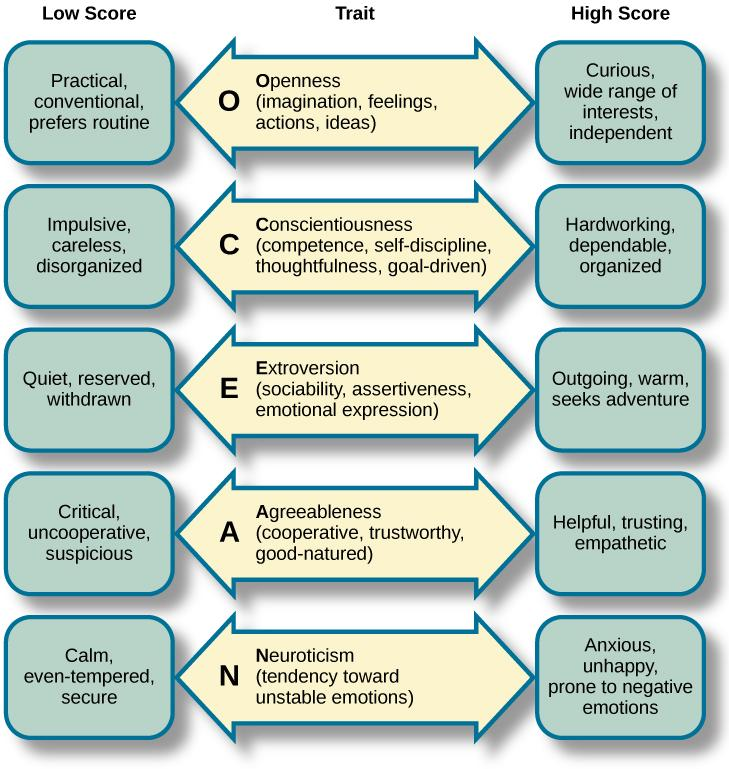
\includegraphics[width=\textwidth]{figures/big-5-personality.jpeg}
  \caption{The big five personality traits. [57]}
  \label{fig:big5}
\end{figure}
%
As shown in Figure \ref{fig:big5} \cite{big5-image}, the Big Five  represent the personality traits as a spectrum where it identifies what is considered a low and high score for each trait. \\

\textbf{Openness} refers to being intellectually curious, innovative, and appreciate art and beauty. People who score high in openness also like theories that explains how things work, are more adventurous, imaginative, aware of their feelings and have a high level of insight as well as being attracted to the idea of abstract thinking \cite{big-five-john1999big}. An open person uses a lot of time in his/her imagination fantasizing and is creative. Additionally, people with high scores in openness are characterized to dislike routine. They are flexible and persevere certain tasks. These characteristics are generally considered positive for a workplace environment. Individuals with a high score in this trait are more often promoted to leadership positions than those who have a low in openness. Openness is fairly stable over time although it shows to increase as people grow older. People with low score in openness dislike change and like routines. They make safe decisions and have low tolerance for a lot of varying ideas. In addition, they have a restricted range of interest meaning a lower levels of intellectual curiosity. Openness is associated with expressing a mixture of positive and negative emotions \cite{openness1-BARFORD2016118}. From a language perspective, people who use more articles in their texts (e.g. words such as ‘the’, ‘an’ and ‘a’), indicate that those people are highly intellectual and open to experience \cite{openness2-fast2008personality}. \\

\textbf{Conscientiousness} is the trait of being conscientious and is the tendency to be able to control impulses and plan out activities carefully. People who score high in conscientiousness prioritize well, are organized, and are good at analyzing situations. They think through situations carefully and have good orientation toward detail \cite{big-five-john1999big}. They like a set schedule and are considered prudent. Individuals who are high in conscientiousness are reliable and is one of the biggest reasons employers favor a high score in this trait. Generally, they are considered higher performing employers. Also, they tend to be more successful in terms of their career. Conscientious people have a lot of self-discipline, less negative interaction with the criminal justice system. They do better in school and in general are more concerned with appearances. Their work environments are more organized and clean. They are also concerned how others will perceive that. As a results, there are many desirable outcomes that occur as a result of being conscientious. At the other side of the spectrum, a person with low conscientiousness is more likely to be disorganized and act on impulses. In self-narratives, people with high score in conscientiousness are more likely to discuss achievements than people with a low score \cite{conscientiousness1-HIRSH2009524}. This trait goes down in adolescence and increases from that point on as individuals grow older. \\

The \textbf{extraversion} trait entail where somebody gets their energy from and how much stimulation that is needed to be functional. Someone who is high in extroversion get their energy from social interactions and social relationships \cite{big-five-john1999big}. They like to be the center of attention and are more talkative. They have many acquaintances but not many close friends and sometimes. Also extroverts struggle with deep analysis. A lower score in this trait, referred to as introvert, has many close friends but not many acquaintances. They do not get energy from social interactions but rather drain energy from this setting. Introverts like being alone, having quiet time and thinking. Extraversion is connected with positive affect and uses more positive words in their language compared to introverts \cite{extraversion1-komulainen2014effect} \cite{extraversion2-pennebaker1999linguistic}. However, it is not stated that introverts express negative emotions. Behaviors such as shyness and sadness is often incorrectly connected with introverts. For example, introverts may not reach out and initiate contact with people but be friendly if someone approached them. When it comes to the work environment, a person with high score in extraversion is linked to leadership roles because extroverts tend to be more assertive individuals and they are more likely to put themselves in dominant positions and take charge.  \\

\textbf{Agreeableness} is a trait where people have an increased amount to care for other people and taking an interest in other people. People who scores high in agreeableness  have a higher degree of empathy, both cognitive and affective empathy. They tend to look for ways to compromise and generally someone who is agreeable is friendly. On the other side of the spectrum, someone who is disagreeable is more competitive and have lower interest in other people. Disagreeable people have a lower degree of empathy and are generally skeptical of people's motives. This can result in an individual being not liked because they appear suspicious and unfriendly. These traits have advantages in certain places. Therefore, agreeableness is associated with higher positive emotions and lower negative effect \cite{personality_emotions_link}. \\

\textbf{Neuroticism} is characterized by emotional dysregulation or high emotional reactivity \cite{big-five-john1999big}. Someone who scores high in neuroticism would have a more negative response to frustration. It is also a tendency to experience negative feelings in particular anger, frustration, and anxiety. Self-esteem is usual an issue for individuals when they are high in neuroticism. With a high score follows certain risks including physical an mental health problems, feeling low satisfaction, and poor work performance. With low score of neuroticism is emotional stability and not being upset as easily. Low neurotic people experience and express fewer negative feelings. However, a low score does not indicate more positive emotions as compared to extraversion. Neuroticism decreases as individuals grow older. If a person with high neuroticism has high conscientiousness, the person can channel their anxiety in a productive way. 






